\documentclass[border=10pt]{standalone}
\usepackage{fontspec}
\setmainfont{DejaVu Sans}
\usepackage{tikz}
\usetikzlibrary{arrows.meta}

\tikzset{
  msg/.style={-{Stealth[round]}, thick, draw=blue!55!black},
  ret/.style={-{Stealth[round]}, thick, dashed, draw=black!55},
  mlbl/.style={midway, above, font=\sffamily\scriptsize, fill=white, inner sep=1.5pt},
}

\begin{document}
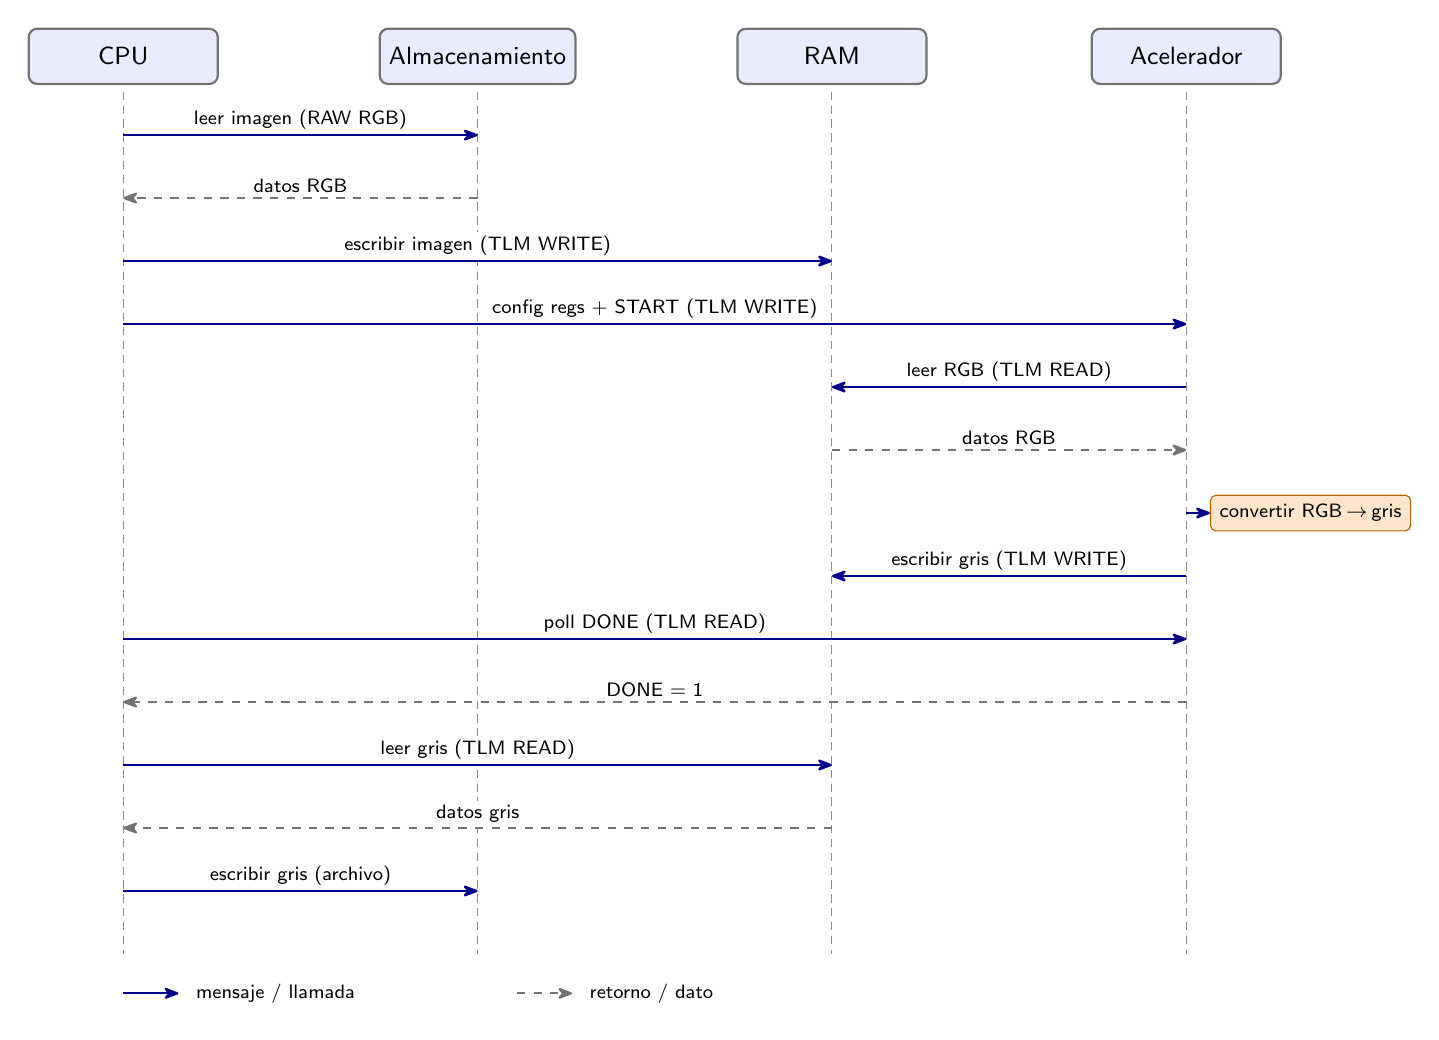
\begin{tikzpicture}
% --- lifelines + cabeceras ---
\foreach \x/\name in {0/CPU, 4.5/Almacenamiento, 9/RAM, 13.5/Acelerador} {
  \node[draw=black!55, thick, rounded corners=3pt, fill=blue!8,
        minimum width=2.4cm, minimum height=0.7cm, font=\sffamily\small] at (\x,0) {\name};
  \draw[densely dashed, black!45] (\x,-0.45) -- (\x,-11.4);
}

% --- mensajes ---
\draw[msg] (0,-1.0)  -- (4.5,-1.0)  node[mlbl]{leer imagen (RAW RGB)};
\draw[ret] (4.5,-1.8) -- (0,-1.8)   node[mlbl]{datos RGB};
\draw[msg] (0,-2.6)  -- (9,-2.6)    node[mlbl]{escribir imagen (TLM WRITE)};
\draw[msg] (0,-3.4)  -- (13.5,-3.4) node[mlbl]{config regs + START (TLM WRITE)};
\draw[msg] (13.5,-4.2) -- (9,-4.2)  node[mlbl]{leer RGB (TLM READ)};
\draw[ret] (9,-5.0)  -- (13.5,-5.0) node[mlbl]{datos RGB};

% accion interna del acelerador
\draw[msg] (13.5,-5.8) -- (13.8,-5.8);
\node[draw=orange!75!black, fill=orange!20, rounded corners=2pt,
      font=\sffamily\scriptsize, anchor=west] at (13.8,-5.8) {convertir RGB\,$\to$\,gris};

\draw[msg] (13.5,-6.6) -- (9,-6.6)  node[mlbl]{escribir gris (TLM WRITE)};
\draw[msg] (0,-7.4)  -- (13.5,-7.4) node[mlbl]{poll DONE (TLM READ)};
\draw[ret] (13.5,-8.2) -- (0,-8.2)  node[mlbl]{DONE = 1};
\draw[msg] (0,-9.0)  -- (9,-9.0)    node[mlbl]{leer gris (TLM READ)};
\draw[ret] (9,-9.8)  -- (0,-9.8)    node[mlbl]{datos gris};
\draw[msg] (0,-10.6) -- (4.5,-10.6) node[mlbl]{escribir gris (archivo)};

% leyenda
\draw[msg] (0,-11.9) -- (0.7,-11.9);
\node[anchor=west, font=\sffamily\scriptsize] at (0.8,-11.9) {mensaje / llamada};
\draw[ret] (5,-11.9) -- (5.7,-11.9);
\node[anchor=west, font=\sffamily\scriptsize] at (5.8,-11.9) {retorno / dato};
\end{tikzpicture}
\end{document}
